%! TEX program = lualatex
\documentclass[a4paper, 12pt]{article}

\usepackage[margin=2.5cm]{geometry}
\usepackage{microtype}
\usepackage{indentfirst}
\usepackage{polyglossia}
\usepackage[colorlinks=true, allcolors=black]{hyperref}
\usepackage{graphicx}
\usepackage[font=footnotesize, labelfont=bf]{caption}
\usepackage{wrapfig}
\usepackage{amsmath}
\usepackage{amsfonts}
\usepackage{mathrsfs}
\usepackage{icomma}
\usepackage{titling}
\usepackage{enumitem}

\setdefaultlanguage{romanian}

\addto\captionsromanian{
    \renewcommand{\figurename}{Fig.}
}

% Enable usage of \\ in sections
\pdfstringdefDisableCommands{%
    \def\\{}%
}

\newcommand{\mktitle}{%
    \noindent
    {\small\theauthor}

    \begin{center}
        \LARGE\thetitle
    \end{center}
}
\newcommand{\parbreak}{\vspace{1cm}}
\newcommand{\unit}[1]{~ \mathrm{#1}}

\title{Dualismul undă-corpuscul. Ipoteza de Broglie}
\author{Andrei Ancuța \\ clasa a XII-a B \\
Liceul Teoretic de Informatică „Grigore Moisil”, Iași}

\begin{document}

\mktitle
\tableofcontents

\section{Cinematica relativistă. Consecințele cinematice ale transformărilor Lorentz}

\subsection{Contracția relativistă a lungimilor}

În mecanica clasică, conform transformărilor Galilei, se aplică invarianța
intervalului spațial, adică dimensiunile corpurilor rămân constante la
trecerea de la un SRI la altul.

Intervalul temporal este de asemenea considerat invariant la trecerea
de la un SRI la altul.

Însă timpul și spațiul nu mai pot fi considerate mărimi absolute în teoria
relativității creată de Einstein.

Prin trecerea de la un SRI la altul, dimensiunile longitudinale ale corpurilor
suferă modificări.

\parbreak

De exemplu, considerăm un corp de formă liniară, precum o riglă, aflată pe axa
$Ox$ în repaus și având lungimea $l_0$ în sistemul S, numit
\emph{sistem de referință propriu} (SRP). Putem exprima $l_0$ prin diferența
absciselor capetelor sale:
\[ l_0 = x_2(t) - x_1(t) \]

\newcommand{\betalorentzradical}{\sqrt{1 - \beta^2}}

Mai departe, măsurăm lungimea riglei în sistemul de referință inerțial $S'$,
care are o mișcare de translație uniformă de-a lungul $Ox$ cu viteza $V$ față de $S$.
Fie $x_1'$ și $x_2'$ abscisele riglei măsurate la același moment de timp $t'$,
măsurat cu un ceas solidar cu $S'$. Conform transformărilor Lorentz, obținem
\[
    l_0 = x_2 - x_1
    = \frac{x_2' + Vt'}{\betalorentzradical} - \frac{x_1' + Vt'}{\betalorentzradical}
    = \frac{x_2' - x_1'}{\betalorentzradical} = \frac{l'}{\betalorentzradical},
\]
unde am notat \( \beta = \frac{V}{c} \). De aici rezultă
\[ l' = l_0 \betalorentzradical \]

Se observă că lungimea $l'$ măsurată în $S'$ este mai mică decât lungimea
proprie $l_0$. Rigla a rămas identică cu ea însăși, însă rezultatul măsurării
lungimii diferă de la un SRI la altul.

\parbreak

Dimensiunile transversale ale corpurilor nu se modifică: \( y' = y \) și \( z' = z \).
Astfel, volumul corpului se modifică doar în direcția mișcării:
\[ \mathscr{V}_0 = xyz \]
\[ \mathscr{V}' = x'y'z' = x\lorentzradical yz = \mathscr{V}_0 \lorentzradical \]

\begin{wrapfigure}{r}{0.4\textwidth}
    \centering
    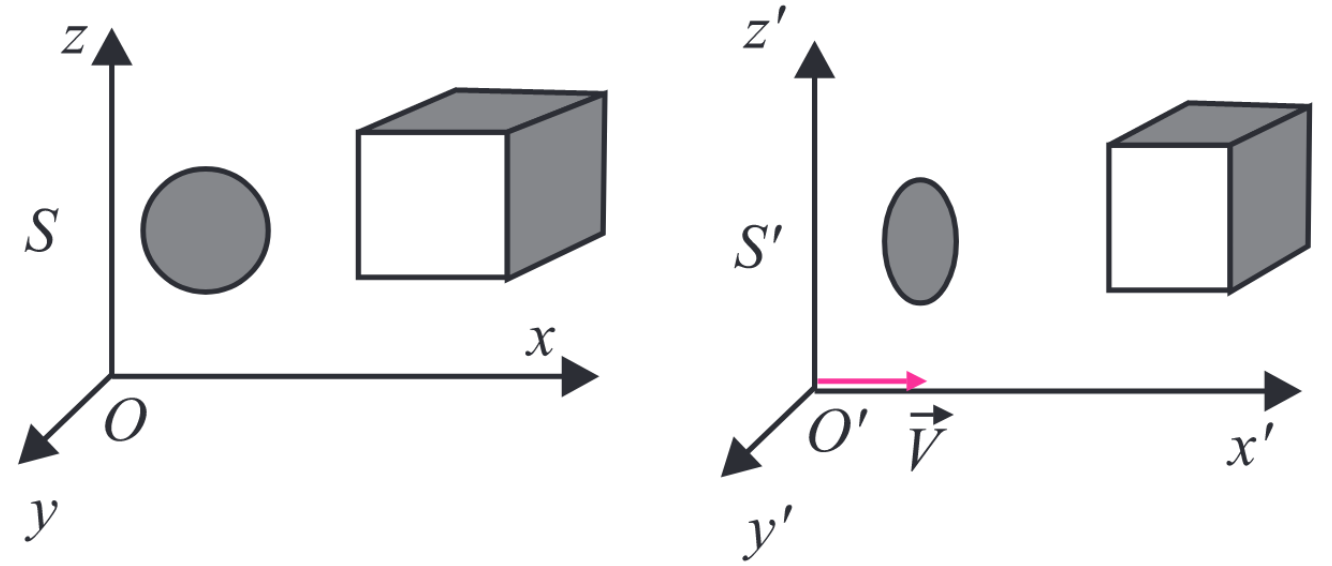
\includegraphics[width=0.4\textwidth]{fig/turtit}
    \caption{Sfera se turtește, iar cubul \linebreak se transformă în paralelipiped}
\end{wrapfigure}

Privind o sferă dintr-un sistem de referință față de care se mișcă, aceasta
apare turtită în direcția mișcării. Un cub devine un paralelipiped.

Aceste modificări reprezintă forma reală a obiectelor, nu doar ceea ce vede un
observator. Atunci când observăm un obiect în mișcare rapidă, în realitate
înregistrăm fotonii care ajung pe retină. Fotonii nefiind emiși
simultan de toate punctele corpului, ochiul percepe o imagine deformată.

Dacă viteza corpului ar fi \( V = c \), dimensiunea sa longitudinală s-ar reduce
la zero, corpul degenerând într-un plan transversal față de $Ox$.

Prin urmare, concepția spațiului absolut \( \left( l' = l_0 \right) \) este
înlocuită în teoria relativistă de concepția spațiului relativ, reprezentată
de relația \( l' = l_0 \lorentzradical \). Orice dimensiune poate fi cunoscută
numai în mărime relativă.

Pentru \( V \rightarrow 0 \), avem \( \lorentzradical \rightarrow 1 \) și deci
relația clasică \( l' = l_0 \).

Pentru \( V > c \), radicalul lui Lorentz devine imaginar, iar noțiunea de lungime
își pierde sensul.

\pagebreak

\subsection{Dilatarea relativistă a timpului}
Pe semiaxa $Ox$ a sistemului $S$, considerăm un eveniment temporar cu durata
\[ \tau_0 = t_2(x) - t_1(x) \]

$\tau_0$ mai este numit și timp propriu.

Durata acestui eveniment, măsurată în sistemul $S'$, aflat în mișcare față de
$S$, este egală cu diferența momentelor respective în $S'$ luate pentru aceeași
abscisă $x$:
\[ \tau' = t_2'(x) - t_1'(x) \]

Din \( t' = \dfrac{t - \frac{Vx}{c^2}}{\lorentzradical} \) rezultă:
\[
    \tau'
    = \frac{t_2 - \frac{Vx}{c^2}}{\lorentzradical}
    - \frac{t_1 - \frac{Vx}{c^2}}{\lorentzradical}
    = \frac{t_2 - t_1}{\lorentzradical} = \frac{\tau_0}{\lorentzradical} > \tau_0
\]

Prin urmare, durata $\tau'$ măsurată în sistemul $S'$ a unui eveniment într-un
punct aflat în mișcare față de $S'$ este mai mare decât durata $\tau_0$
măsurată în sistemul $S$, față de care punctul se află în repaus:
\( \tau' > \tau_0 \).

De aici rezultă că durata unui eveniment este minimă măsurată față de sistemul
de referință propriu.

\parbreak

%Dependența intervalului de timp de sistemul de referință nu este intuitivă în
%comparație cu fenomenele pe care le observăm zi de zi în regim nerelativist,
%când \( V \ll c \).
%
%Un exemplu îl reprezintă prezența miuonilor la nivelul solului sau mării.
%Miuonii, care apar în atmosferă la altitudini de 10 km, datorită razelor
%cosmice ce pătrund în atmosfera planetei, au un timp de viață propriu -- cel
%măsurat în SRP -- extrem de scurt, \( \tau_0 = 2,2 \cdot 10^{-6} ~ \mathrm{s} \).
%Având viteza \( V = 2,994 \cdot 10^8 \) m/s (valoare apropiată de viteza
%luminii), din calculul nerelativist al distanței rezultă că un miuon ar putea
%parcurge doar \( V\tau_0 = 658,7 \) m în intervalul de timp propriu, distanță
%insuficientă pentru a ajunge la nivelul solului.  Deoarece observația se face
%în raport cu Pământul, trebuie să luăm în considerație intervalul de timp
%măsurat față de Pământ:
%
%\[
%    \tau = \frac{\tau_0}{\lorentzradical}
%    = \frac{2,2 \cdot 10^{-6}}{\sqrt{1 - \left( \frac{2,994}{2,9979} \right)^2}}
%    = 43,14 \cdot 10^{-6} ~ \mathrm{s}
%\]
%
%Calculând acum distanța parcursă de miuon față de Pământ, obținem:
%\[ D = c\tau = 12,933 ~ \mathrm{km} \]
%
%Rezultă că miuonul poate fi reperat la nivelul solului și chiar al mării.

Pentru \( V \ll c \) se obține \( \tau = \tau_0 \), ca în mecanica clasică.

Pentru \( V \rightarrow c \), dimensiunile longitudinale ale corpurilor tind
către 0, iar intervalul de timp către infinit.

Pentru \( V = c \), corpul este redus la un plan transversal pe direcția
mișcării, iar intervalul de timp devine infinit.

Pentru \( V > c \), transformările Lorentz devin imaginare și își pierd
sensul fizic, demonstrând că viteza luminii în vid nu poate fi atinsă de
corpuri.

În concluzie, pentru un observator aflat în mișcare față de locul unde se
produce un fenomen, acesta se desfășoară mai lent decât pentru un observator
aflat în repaus față de eveniment.

Simultaneitatea a două evenimente este de asemenea dependentă de sistemul de
referință față de care este descrisă mișcarea. Două evenimente simultane în
$S$ nu sunt simultane în $S'$.

Fie două evenimente simultane în $S$ în punctele $x_1$ și $x_2$ la momentul
$t$. În $S'$, aflat în mișcare față de $S$, vom măsura timpii:
\begin{equation*}
    \begin{aligned}[t]
        t_1'(x_1) = \frac{t - \frac{Vx_1}{c^2}}{\lorentzradical}
    \end{aligned}
    \qquad\qquad\qquad
    \begin{aligned}[t]
        t_2'(x_2) = \frac{t - \frac{Vx_2}{c^2}}{\lorentzradical}
    \end{aligned}
\end{equation*}

Observate din $S'$, evenimentele nu mai apar simultane, cu excepția cazului în
care \( x_1 = x_2 \), adică atunci când evenimentele coincid.

Rolul principal al teoriei relativității este de a stabili
\emph{invarianții relativiști}: mărimi cu proprietatea de a rămâne invariante
la trecerea de la un SRI la altul. Printre aceștia se numără constantele
universale, sarcina electrică, mărimile măsurate față de SRP etc.



\section{Ipoteza de Broglie. Difracția electronilor. Aplicații}

Analog cu dualismul undă-corpuscul în cazul undelor electromagnetice, Louis de Broglie asociază oricărei microparticule în mișcare cu energia $E$ și impulsul $p$ o undă caracterizată prin frecvența $\nu$ și lungimea de undă $\lambda$, cu relațiile dintre mărimi
\[
    E = h \nu
    \begin{Bmatrix}
        \nu & \lambda \\
        E   & p
    \end{Bmatrix}
    p = \frac{h}{\lambda}
\]

De Broglie a presupus că lungimea de undă a undelor asociate microparticulelor
trebuie să fie dată tot de relația \( \lambda = \frac{h}{p} \), unde $p$ este
impulsul microparticulei.

\parbreak

Ipoteza de Broglie afirmă că oricărei microparticule care posedă un impuls $p$
i se poate asocia în mod formal o undă cu lungimea de undă
\( \lambda_B = \frac{h}{p} \), numită lungime de undă de Broglie.

Undelor electromagnetice le sunt asociați fotonii, care nu au masă de repaus.
Analog, undele de Broglie sunt asociate particulelor cu masă de repaus:
electroni, protoni, neutroni, particule \alpha, molecule de hidrogen. În
concluzie, radiația electromagnetică are proprietăți ondulatorii și
corpusculare, asemenea radiației corpusculare.

\subsection*{Experimentul Davisson-Germer}

Fizicienii Davisson și Germer au confirmat experimental ipoteza de Broglie,
demonstrând că electronii în mișcare prezintă proprietăți ondulatorii, prin
generarea fenomenelor de difracție însoțite de interferență.

\begin{wrapfigure}{r}{0.45\textwidth}
    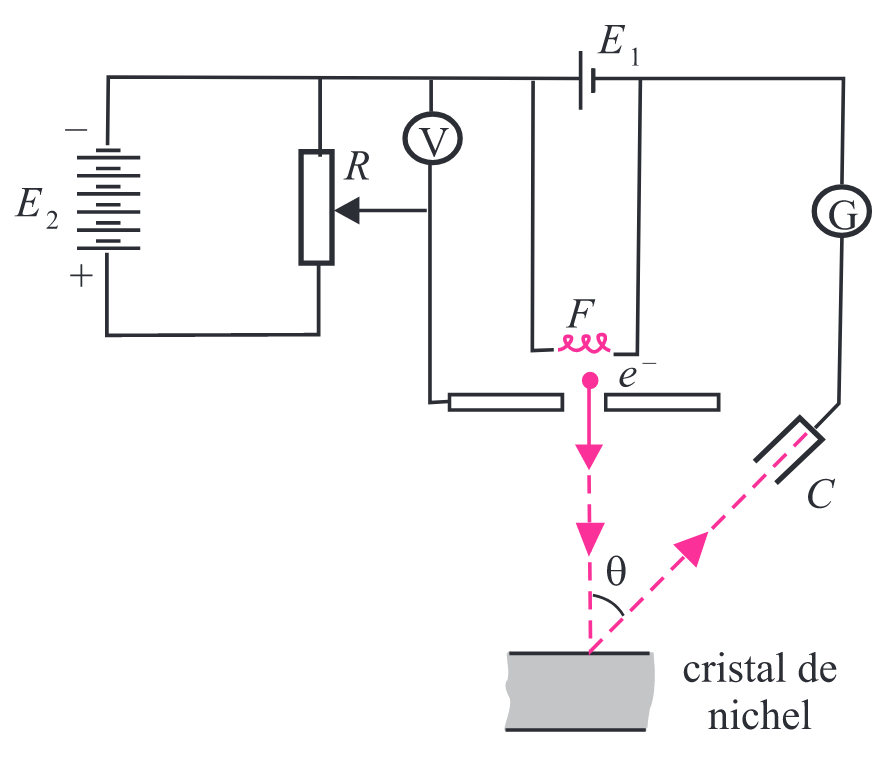
\includegraphics[width=0.45\textwidth]{fig/davisson_germer}
    \caption{Schema experimentului}
\end{wrapfigure}

Filamentul $F$, alimentat de sursa $E_1$, emite electroni care sunt accelerați
într-un tun electronic, alimentat de sursa $E_2$. Tensiunea de accelerare $U$
este controlată de reostatul $R$ și măsurată cu voltmetrul $V$.

Fasciculul monoenergetic de electroni, numit \emph{monocromatic}, care iese din
tunul electronic, are energia:
\begin{equation}
    \frac{m_e v^2}{2} = eU \label{eq:1}
\end{equation}

Fasciculul cade pe un monocristal de nichel, iar fasciculul difractat este
captat de un cilindru Faraday $C$ colector. Curentul de electroni este măsurat
de galvanometrul $G$.

Se observă că intensitatea fasciculului de electroni difractați prezintă maxime
și minime în funcție de $U$ și unghiul de incidență $\theta$.

Din relația \eqref{eq:1} rezultă \( v = \sqrt{\frac{2eU}{m_e}} \).

În cazul nerelativist avem impulsul \( p = m_e v = \sqrt{2em_e U} \), iar
lungimea de undă de Broglie asociată este:
\[
    \lambda_B = \frac{h}{p} = \frac{h}{\sqrt{2em_e} U}
    = \frac{h}{\sqrt{2em_e}} \cdot \frac{1}{\sqrt{U}}
    = \frac{12,23 \cdot 10^{-10}}{\sqrt{U}}
\]

Pentru un potențial de accelerare \( V = 54 \unit{V} \), lungimea de undă
este de același ordin de mărime cu lungimea de undă a radiației X:
\begin{equation}
    \lambda_B = \frac{12,23 \cdot 10^{-10}}{\sqrt{54}}
    = 1,664 \cdot 10^{-10} \unit{m} \label{eq:2}
\end{equation}

Fenomenele de difracție pot fi observate când unda interacționează cu o „rețea
de difracție” a cărei constantă de rețea are dimensiunile comparabile cu
lungimea de undă (\( 10^{-10} \unit{m} \)).

\begin{wrapfigure}{r}{0.45\textwidth}
    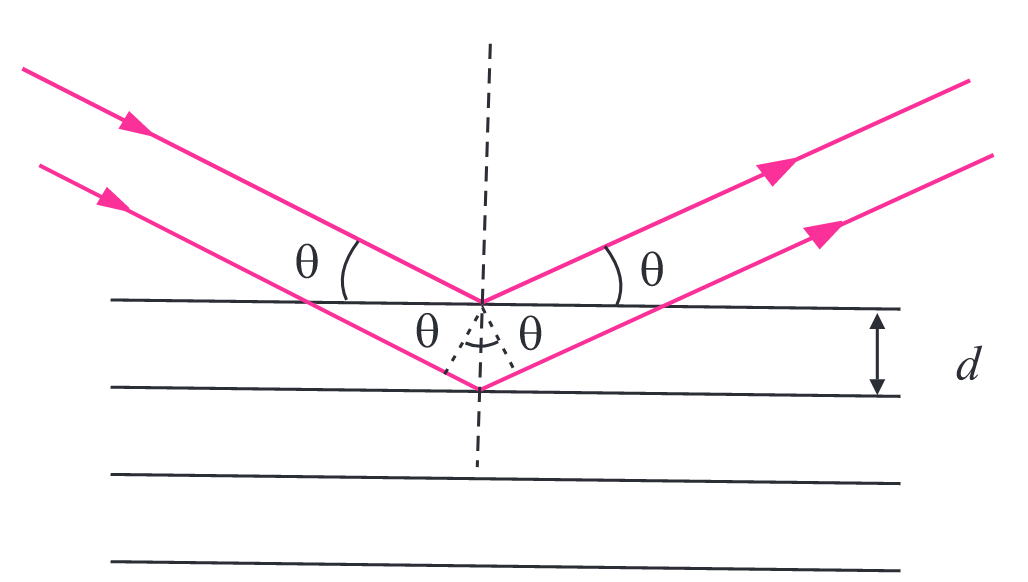
\includegraphics[width=0.45\textwidth]{fig/monocristal}
    \caption{Difracția razelor X pe un monocristal}
\end{wrapfigure}

Atomii monocristalului sunt așezați ordonat, distanța dintre doi atomi vecini
fiind de ordinul \( 10^{-10} \unit{m} \). Această aranjare regulată în nodurile
rețelei cristaline conferă proprietățile unei rețele de difracție
tridimensionale.

În urma studierii difracției razelor X pe monocristale, Bragg a stabilit că
intensitatea fasciculului difractat trece prin valori maxime în cazul:
\begin{equation}
    2d\sin\theta = k\lambda, k \in \mathbb{N^*} \label{eq:3}
\end{equation}
unde:
\begin{itemize}
    \item $\theta$ este unghiul format de planul reticular cu direcția fasciculului incident, respectiv cel difractat.
    \item $d$ este constanta rețelei, adică distanța dintre două plane reticulare.
    \item $\lambda$ este lungimea de undă a radiației.
    \item $2d\sin\theta$ este diferența de drum dintre razele difractate de două plane reticulare vecine.
\end{itemize}

În cazul în care particulele suferă o difracție, se aplică relația
\eqref{eq:3}. Pentru \( d = 0,91 \cdot 10^{-10} \unit{m} \), $k = 1$,
$U = 54 \unit{V}$, tensiune la care se obține primul maxim pentru
$\theta = 65^\circ$, se obține:
\begin{equation}
    \lambda_B = 2d\sin\theta = 2 \cdot 0,91 \cdot 10^{-10} \cdot 0,906 = 1,65 \cdot 10^{-10} \unit{m} \label{eq:4}
\end{equation}

Valorile obținute în relațiile \eqref{eq:2} și \eqref{eq:4} se află în concordanță, confirmând că
electronii în mișcare au proprietăți ondulatorii.

Lungimea de undă de Broglie este invers proporțională cu masa particulelor cărora le este asociată.

Microparticulele, numite \emph{particule cuantice}, sunt radical diferite de
particulele clasice, supunându-se unor legi specifice. Nu sunt nici particule,
nici unde în sens clasic, comportamentul lor reflectând dualismul
corpuscul-undă.

Deși unda de Broglie asociată microparticulelor nu este o undă în sensul clasic
al cuvântului, este folosită această noțiune.

La nivel macroscopic, un corpuscul nu poate avea proprietăți ondulatorii, iar
unda nu poate fi concepută ca un flux de particule discrete. Particulele
cuantice aparțin însă nivelului cuantic, fiind radical diferite de unde și
corpusculi. De exemplu, ele nu au traiectorii.

Asupra sistemelor cuantice putem face doar afirmații statistice.

\subsection*{Microscopul electronic}

Microscopul electronic este o aplicație a ipotezei lui de Broglie. Un
fasciculul de electroni cade pe un preparat și îl traversează, variațiile de
grosime ale preparatului devenind variații de intensitate a fasciculului.
Utilizând câmpuri electrice sau magnetice, traiectoriile electronilor sunt
asemănătoare traiectoriilor razelor de lumină dintr-un microscopic optic.

În cazul microscopului optic, pentru a distinge două puncte, distanța dintre
ele trebuie să fie mai mare decât lungimea de undă a luminii folosite, adică
mai mare decât zecimi de microni (puterea de separare).

În locul lentilelor optice se găsesc bobinele parcurse de curent electric
(\emph{lentile magnetice}) sau electrozii încărcați electric
-- \emph{lentile electrice} -- ce pot focaliza și defocaliza un fascicul de
electroni.

\parbreak

\begin{minipage}{0.6\textwidth}
    \captionsetup{type=figure}
    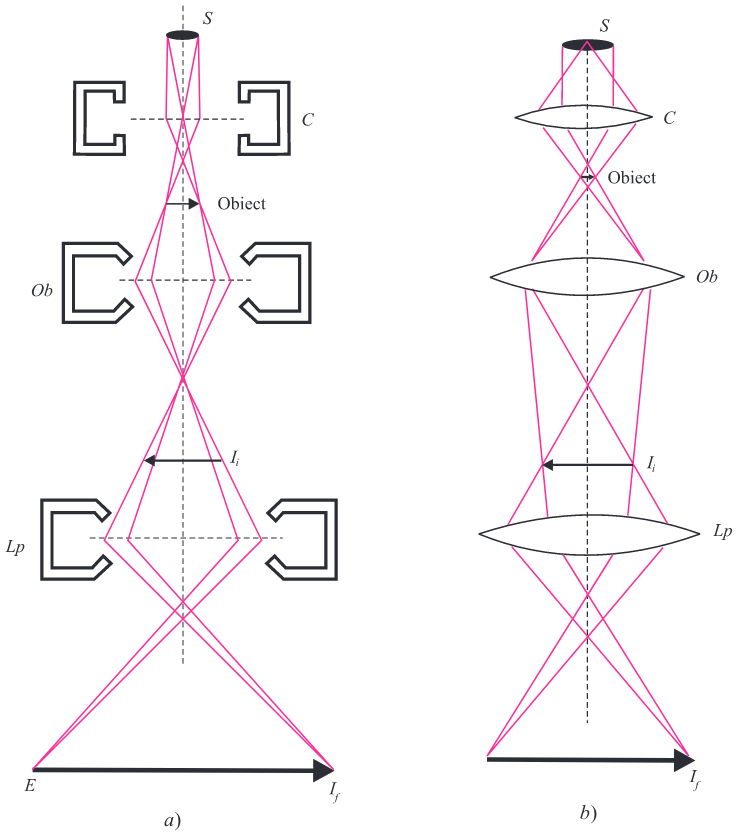
\includegraphics[width=\textwidth]{fig/microscop}
    \caption{Schema microscopului electronic și a microscopului optic}
\end{minipage}%
\hspace{0.5cm}%
\begin{minipage}{0.3\textwidth}
    \begin{itemize}[left=0pt,label=]
        \item $S$ -- sursa de electroni (a) sau lumină (b)
        \item $C$ -- condensator
        \item $Ob$ -- obiectiv
        \item $I_i$ -- imagine intermediară
        \item $Lp$ -- lentilă de proiecție
        \item $I_f$ -- imagine finală
        \item $E$ -- ecran fluorescent
    \end{itemize}
\end{minipage}

\parbreak

Datorită lungimii de undă mult mai mici a undelor asociate electronilor,
puterea de separare a microscopului electronic este mult mai mare decât a
microscopului optic. Transformarea imaginii în una luminoasă se realizează cu
ajutorul unui ecran fluorescent.

Probele examinate trebuie să fie sub formă de pelicule foarte subțiri, din
cauza puterii de pătrundere mici a electronilor.

Au fost construite și microscoape protonice și ionice, care pot mări de 10-15
ori mai mult decât un microscop electronic.


\clearpage

\section*{Bibliografie}
\begin{itemize}
    \item Manualul de fizică pentru clasa a XII-a, F1 \\
        Cleopatra Gherbanovschi, Nicolae Gherbanovschi \\
        Editura NICULESCU ABC \\
        2016
\end{itemize}

\end{document}
